\section{Results}\label{sec:results}

%Här kan du till exempel presentera resultat av experiment, bevis, analys av data etc. Dina resultat måste beskrivas så tydligt att en läsare kan bedöma dem.  Du ska också förklara och analysera resultaten.

The results so far is divided up in two relevant subsections where the first handles the input inference test and the second handles the 3D reconstruction using \aruco corners.
\subsection{OpenPose output inference results}%
\label{sub:res:op_inference}



%----------------------------
\begin{table}[htb]
    \begin{center}
    \begin{minipage}{0.4\textwidth}
        \begin{center}
            \input{../results/error_degdf_df.latex}
        \end{center}
        \caption[Degrees of freedom human vs openpose]{The degrees of freedom for human and \openpose is due to the quite limited dataset not in most cases not statistically viable but perhaps it cold work as a marker.}
        \label{tab:results:degfreedom}
    \end{minipage}
    \begin{minipage}{0.4\textwidth}
        \begin{center}
            \input{../results/direction_degdf_df.latex}
        \end{center}
        \caption[Directional degrees of freedom]{The directional degrees of freedom is a bit better because it do not care about the labels, just the total error for that direction. }
        \label{tab:results:dirdegfreedom}
    \end{minipage}
    \end{center}
\end{table}
%----------------------------
\begin{table}[htb]
    \begin{center}
        \input{../results/ftest_pos_df.latex}
    \end{center}
    \caption{The directional results from F-test and T-test}
    \label{lab:results:human_lable}
\end{table}
%----------------------------
\begin{table}[htb]
    \begin{center}
        \input{../results/error_df.latex}
    \end{center}
    \caption[Results in image domain]{The error results for the human vs \openpose in the image domain. Observe the large variance in the forth column that suggests that \openpose have problem finding the correct solution for that label. It can also be observed that the half of the data in comparison with the human is missing from \openpose columns thus indicating again that it could not find a solution to that label.}
    \label{lab:results:human_vs_openpose}
\end{table}
%----------------------------
\begin{table}[htb]
    \begin{center}
        \input{../results/ftest_pds.latex}
    \end{center}
    \caption{Datasets}
    \label{tab:results:human}
\end{table}


\subsection{3D reconstruction using Aruco}%
\label{sub:res:3drec}
\begin{figure}
\begin{center}
    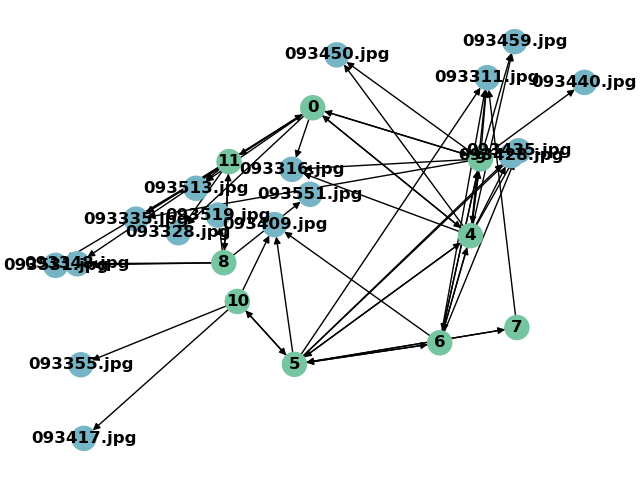
\includegraphics[scale=0.6]{results/atlas.png}
\end{center}
\caption[Results from camera mapping]{Reconstructing the camera pose from the images using Dijkstras algorithm  data proved to be a harder problem then initially thought. Ni this results the green numbered nodes seams to find the correct location, but the input camera view nodes in blue do not.}
\label{fig:results:mapreconstruction}
\end{figure}


